\documentclass[10pt]{article}
\usepackage[a4paper,margin=18mm,bottom=20mm,footskip=9mm]{geometry}
\usepackage{xeCJK}
\setCJKmainfont{Noto Serif CJK SC}[ItalicFont=Noto Serif CJK SC, BoldFont=Noto Serif CJK SC SemiBold]
\setCJKsansfont{Noto Sans CJK SC}[BoldFont=Noto Sans CJK SC Medium]
\usepackage{cvstyle}
\xeCJKsetup{CJKspace=false}
\linespread{1.18}

\setlength{\datecol}{26mm}
\setlength{\amountcol}{36mm}
\renewcommand{\sectionlabel}[1]{{\addfontfeature{LetterSpace=10}#1}}
\renewcommand{\footleft}{Jidu Yu\ 个人简历\,·\,更新于 2026 年 10 月}
\renewcommand{\footright}{第 \thepage\ 页\,/\,共 \pageref*{LastPage} 页}
\renewcommand{\fact}[2]{{\sffamily\footnotesize\color{muted}#1}\ {\color{ink}#2}}

% generated by build.py from _data/publications.yml -- do not edit
\newcommand{\GSCitations}{337}
\newcommand{\GSh}{10}
\newcommand{\GSiten}{11}
\newcommand{\GSupdated}{Oct 2026}
\newcommand{\GSurl}{https://scholar.google.com/citations?user=AgtKCIIAAAAJ}
\newcommand{\NJournal}{20}
\newcommand{\PubsJournal}{\item[J20] Chen X.Y., Zhao J.D.\corr{}, \textbf{Yu J.D.} (2026). The infiltration paradox: Pore-gas pressure controls on early slope failure during rapid hydraulic loading. \emph{Engineering Geology}, 109124.\pubdoi{https://doi.org/10.1016/j.enggeo.2026.109124}{doi:10.1016/j.enggeo.2026.109124}
\item[J19] \textbf{Yu J.D.}, Zhao J.D. (2026). A virtual heat flux method for simple and accurate Neumann thermal boundary imposition in the material point method. \emph{International Journal for Numerical Methods in Engineering}, 127(12), e70371.\pubdoi{https://doi.org/10.1002/nme.70371}{doi:10.1002/nme.70371}
\item[J18] Liu Y.S., Shen C.M.\corr{}, Liu S.H., \textbf{Yu J.D.}, Liu Y.C., Li B.W. (2026). Refined constitutive modelling of widely graded granular soils incorporating fractional particle breakage. \emph{Computers and Geotechnics}, 194, 107973.\pubdoi{https://doi.org/10.1016/j.compgeo.2026.107973}{doi:10.1016/j.compgeo.2026.107973}
\item[J17] Zhang C.X., Chen Y.N.\corr{}, \textbf{Yu J.D.}, Yang Z.X., Jardine R.J., Guo N. (2026). Stabilized semi-implicit material point method for hydro-mechanical coupled large deformation soil-structure interaction analyses. \emph{International Journal for Numerical and Analytical Methods in Geomechanics}, 50(9), 3935–3954.\pubdoi{https://doi.org/10.1002/nag.70314}{doi:10.1002/nag.70314}
\item[J16] \textbf{Yu J.D.}\corr{}, Zhao J.D.\corr{}, Liang W.J. (2026). Multiscale modeling of coupled thermo-hydro-mechanical-chemical behavior in hydrate-bearing sediment. \emph{Journal of the Mechanics and Physics of Solids}, 210, 106512.\pubdoi{https://doi.org/10.1016/j.jmps.2026.106512}{doi:10.1016/j.jmps.2026.106512}
\item[J15] \textbf{Yu J.D.}, Zhao J.D.\corr{}, Soga K., Zhao S.W., Liang W.J. (2026). A fully coupled THMC-MPM framework for modeling phase transition and large deformation in methane hydrate-bearing sediment. \emph{Journal of the Mechanics and Physics of Solids}, 206, 106368.\pubdoi{https://doi.org/10.1016/j.jmps.2025.106368}{doi:10.1016/j.jmps.2025.106368}
\item[J14] Liang W.J., Chandra B., \textbf{Yu J.D.}, Yin Z.Y.\corr{}, Zhao J.D. (2025). A total-Lagrangian material point method for fast and stable hydromechanical modeling of porous media. \emph{International Journal for Numerical Methods in Engineering}, 126(19), e70135.\pubdoi{https://doi.org/10.1002/nme.70135}{doi:10.1002/nme.70135}
\item[J13] \textbf{Yu J.D.}, Liang W.J., Zhao J.D.\corr{} (2025). Enhancing dynamic modeling of porous media with compressible fluid: A THM material point method with improved fractional step formulation. \emph{Computer Methods in Applied Mechanics and Engineering}, 444, 118100.\pubdoi{https://doi.org/10.1016/j.cma.2025.118100}{doi:10.1016/j.cma.2025.118100}
\item[J12] \textbf{Yu J.D.}, Zhao J.D.\corr{}, Liang W.J., Zhao S.W. (2024). Multiscale modeling of coupled thermo-hydro-mechanical behavior in ice-bonded granular media subject to freeze-thaw cycles. \emph{Computers and Geotechnics}, 171, 106349.\pubdoi{https://doi.org/10.1016/j.compgeo.2024.106349}{doi:10.1016/j.compgeo.2024.106349}
\item[J11] \textbf{Yu J.D.}, Zhao J.D.\corr{}, Zhao S.W., Liang W.J. (2024). Thermo-hydro-mechanical coupled material point method for modeling freezing and thawing of porous media. \emph{International Journal for Numerical and Analytical Methods in Geomechanics}, 48(13), 3308–3349.\pubdoi{https://doi.org/10.1002/nag.3794}{doi:10.1002/nag.3794}
\item[J10] \textbf{Yu J.D.}, Zhao J.D.\corr{}, Liang W.J., Zhao S.W. (2024). A semi-implicit material point method for coupled thermo-hydro-mechanical simulation of saturated porous media in large deformation. \emph{Computer Methods in Applied Mechanics and Engineering}, 418, 116462.\pubdoi{https://doi.org/10.1016/j.cma.2023.116462}{doi:10.1016/j.cma.2023.116462}
\item[J9] Shen C.M., Liu S.H.\corr{}, Wang L.J., \textbf{Yu J.D.}, Wei H., Wu P. (2022). Packing, compressibility, and crushability of rockfill materials with polydisperse particle size distributions and implications for dam engineering. \emph{Water Science and Engineering}, 15(4), 358–366.\pubdoi{https://doi.org/10.1016/j.wse.2022.07.003}{doi:10.1016/j.wse.2022.07.003}
\item[J8] Shen C.M., \textbf{Yu J.D.}\corr{}, Liu S.H.\corr{}, Mao H.Y. (2021). A unified fractional breakage model for granular materials inspired by the crushing tests of dyed gypsum particles. \emph{Construction and Building Materials}, 270, 121366.\pubdoi{https://doi.org/10.1016/j.conbuildmat.2020.121366}{doi:10.1016/j.conbuildmat.2020.121366}
\item[J7] Shen C.M., Liu S.H.\corr{}, \textbf{Yu J.D.}, Wang L.J. (2021). A simple scale effect model for the volumetric behavior of rockfill materials. \emph{International Journal of Geomechanics}, 21(3), 04020266.\pubdoi{https://doi.org/10.1061/(ASCE)GM.1943-5622.0001939}{doi:10.1061/(ASCE)GM.1943-5622.0001939}
\item[J6] \textbf{Yu J.D.}, Shen C.M.\corr{}, Liu S.H., Cheng Y.P. (2020). Exploration of the survival probability and shape evolution of crushable particles during one-dimensional compression using dyed gypsum particles. \emph{Journal of Geotechnical and Geoenvironmental Engineering}, 146(11), 04020121.\pubdoi{https://doi.org/10.1061/(ASCE)GT.1943-5606.0002371}{doi:10.1061/(ASCE)GT.1943-5606.0002371}
\item[J5] Wang T., Liu S.H.\corr{}, Feng Y., \textbf{Yu J.D.} (2018). Compaction characteristics and minimum void ratio prediction model for gap-graded soil-rock mixture. \emph{Applied Sciences}, 8(12), 2584.\pubdoi{https://doi.org/10.3390/app8122584}{doi:10.3390/app8122584}}
\newcommand{\PubsChinese}{\item[J4] \textbf{Yu J.D.}, Liu S.H.\corr{}, Shen C.M.\corr{}, Mao H.Y. (2022). Breakage and shape evolution of dyed gypsum particles under one-dimensional compression. \emph{Journal of Hohai University (Natural Sciences) (河海大学学报（自然科学版）)}, 50(1), 110–116. (In Chinese)\pubdoi{https://doi.org/10.3876/j.issn.1000-1980.2022.01.016}{doi:10.3876/j.issn.1000-1980.2022.01.016}
\item[J3] Wei H., Shen C.M., Liu S.H., \textbf{Yu J.D.} (2020). Experimental study on compression and crushing characteristics of coarse granular materials considering influence of gradations. \emph{Journal of Hohai University (Natural Sciences) (河海大学学报（自然科学版）)}, 48(2), 182–188. (In Chinese)\pubdoi{https://doi.org/10.3876/j.issn.1000-1980.2020.02.014}{doi:10.3876/j.issn.1000-1980.2020.02.014}
\item[J2] \textbf{Yu J.D.}, Shen C.M.\corr{}, Liu S.H. (2020). Breakage and migration of dyed gypsum particles under one-dimensional compression. \emph{Chinese Journal of Rock Mechanics and Engineering (岩石力学与工程学报)}, 39(5), 1071–1079. (In Chinese)\pubdoi{https://doi.org/10.13722/j.cnki.jrme.2019.0739}{doi:10.13722/j.cnki.jrme.2019.0739}
\item[J1] \textbf{Yu J.D.}, Liu S.H.\corr{}, Wang T., Wei H. (2019). Experimental research on compaction characteristics of gap-graded coarse-grained soils. \emph{Chinese Journal of Geotechnical Engineering (岩土工程学报)}, 41(11), 2142–2148. (In Chinese)\pubdoi{https://doi.org/10.11779/CJGE201911021}{doi:10.11779/CJGE201911021}}
\newcommand{\PubsReview}{\item[R2] Liu X.Y., Gao G., \textbf{Yu J.D.}, Meguid M.A., Zhang F.S. (2026). Micromechanical characterization of fracture evolution in confined jointed rocks using a 3D grain-based model. Submitted to \emph{Rock Mechanics and Rock Engineering}.
\item[R1] \textbf{Yu J.D.}, Chandra B.\corr{}, Wilkes C., Zhao J.D., Soga K. (2025). An elasto-viscoplastic thixotropic model for fresh concrete capturing flow-rest transition. Submitted to \emph{Cement and Concrete Composites}. arXiv:2512.23364.\pubdoi{https://arxiv.org/abs/2512.23364}{arXiv:2512.23364}}
\newcommand{\PubsConference}{\item[C7] \textbf{Yu J.D.}, Zhao J.D.\corr{} (2026). High-fidelity multiscale framework for modelling permafrost thaw-related geohazards. \emph{Proceedings of the 21st International Conference on Soil Mechanics and Geotechnical Engineering (ICSMGE)}, 1743–1746, Vienna, Austria.
\item[C6] \textbf{Yu J.D.}, Zhao J.D.\corr{} (2025). A multiphysics-multiscale MPM-DEM framework for modeling climate-driven geohazards in phase-change granular media. \emph{IX International Conference on Particle-based Methods (Particles 2025)}, 20–22 October 2025, Barcelona, Spain.
\item[C5] \textbf{Yu J.D.}, Zhao J.D.\corr{} (2025). Hybrid explicit-implicit THMC-MPM for modeling phase transition and large deformation in hydrate-bearing sediment. \emph{The 2nd Workshop on Material Point Method \& Extreme Deformation Problems (MPM 2025)}, 12–14 September 2025, Xi'an, China.
\item[C4] \textbf{Yu J.D.}, Zhao J.D.\corr{}, Zhao S.W., Liang W.J. (2024). Thermo-hydro-mechanical coupled material point method for simulating the freeze-thaw behavior of porous media. \emph{16th World Congress on Computational Mechanics and 4th Pan American Congress on Computational Mechanics (WCCM-PANACM 2024)}, July 2024, Vancouver, Canada.
\item[C3] \textbf{Yu J.D.}, Zhao J.D.\corr{}, Zhao S.W., Liang W.J. (2024). Multiphysics simulation of freezing and thawing granular media using material point method. \emph{GeoShanghai International Conference 2024}, May 2024, Shanghai, China. \emph{IOP Conference Series: Earth and Environmental Science}, 1330, 012035.\pubdoi{https://doi.org/10.1088/1755-1315/1330/1/012035}{doi:10.1088/1755-1315/1330/1/012035}
\item[C2] \textbf{Yu J.D.}, Liang W.J., Zhao S.W., Zhao J.D.\corr{} (2023). A semi-implicit MPM for modeling the thermal effect in saturated porous media. \emph{International Symposium on Innovations in Geotechnical Engineering towards Sustainability (IGES 2023)}, Hong Kong, China.
\item[C1] \textbf{Yu J.D.}, Zhao J.D.\corr{}, Zhao S.W., Liang W.J. (2023). An explicit-implicit THM-coupled MPM for saturated porous media. \emph{The 26th Annual Conference of HKSTAM 2023 in conjunction with the 18th Shanghai–Hong Kong Forum on Mechanics and Its Application}, Hong Kong, China, p. 30.}
\newcommand{\PubsThesis}{\item[T1] \textbf{Yu J.D.} (2025). Multiscale modeling of coupled thermo-hydro-mechanical behavior in granular media. Ph.D. thesis, The Hong Kong University of Science and Technology, Hong Kong.\pubdoi{https://doi.org/10.14711/thesis-hdl152441}{doi:10.14711/thesis-hdl152441}}


\begin{document}

% ======================= header with photo =======================
\begin{minipage}[b]{0.62\linewidth}
  {\namefont\fontsize{28}{30}\selectfont\color{ink}Jidu Yu}\\[7pt]
  {\sffamily\fontsize{12.5}{15}\selectfont\color{accent}博士后研究员}\\[3pt]
  {\sffamily\small\color{muted}美国加州大学伯克利分校\ 土木与环境工程系}\\[6pt]
  {\sffamily\small
   邮箱\ \href{mailto:jyubu@connect.ust.hk}{jyubu@connect.ust.hk}\\
   主页\ \href{https://yujidu.github.io}{yujidu.github.io}\\
   \href{https://scholar.google.com/citations?user=AgtKCIIAAAAJ}{Google Scholar}\,·\,%
   \href{https://orcid.org/0000-0002-2311-0603}{ORCID 0000-0002-2311-0603}\,·\,%
   \href{https://github.com/yujidu}{GitHub}}
\end{minipage}\hfill
\begin{minipage}[b]{0.2\linewidth}\raggedleft
  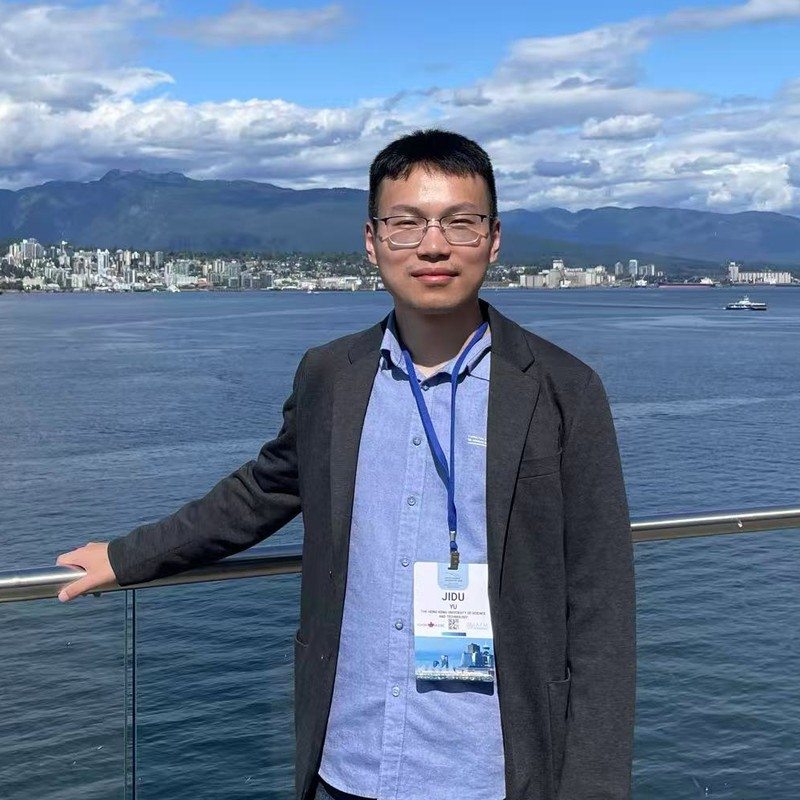
\includegraphics[width=27mm,height=33mm,keepaspectratio=false,trim=73 0 73 0,clip]{photo.jpg}
\end{minipage}

\vspace{7pt}{\color{accent}\rule{\linewidth}{1.3pt}}\vspace{-4pt}

% ======================= research =======================
\section{研究方向}
\cvrow{}{致力于发展极端环境下岩土材料的高保真数值模拟方法，研究热–水–力–化（THMC）多场耦合作用驱动的大变形与破坏过程。}
\vspace{-3pt}
\begin{cvbullets}
  \item 粒子类与混合数值方法：MPM、DEM、MPM-DEM、MPM-FVM
  \item 多相颗粒介质多物理场（THM/C）耦合模拟，如冻土、含水合物沉积物
  \item 气候驱动的地质灾害：冻土融化、降雨诱发滑坡、水合物分解诱发失稳
  \item 极端环境岩土力学：海底、深地与地外环境
  \item 机器学习辅助的多尺度、多物理场模拟
  \item 挤出式材料 3D 打印：流变特性与数值模拟
\end{cvbullets}

% ======================= appointments =======================
\section{工作与访问经历}
\cventry{2026.02 -- 至今}{博士后研究员}
  {美国加州大学伯克利分校\ 土木与环境工程系}
  {\fact{合作导师}{Kenichi Soga 教授}}
\cventry{2025.09 -- 2026.01}{博士后研究员}
  {香港科技大学\ 土木及环境工程学系}
  {\fact{合作导师}{赵吉东 教授}}
\cventry{2024.11 -- 2025.04}{访问博士生}
  {美国加州大学伯克利分校\ 土木与环境工程系}
  {\fact{合作导师}{Kenichi Soga 教授}}
\cventry{2019.07 -- 2019.10}{访问学生}
  {英国伦敦大学学院（UCL）\ 土木、环境与测绘工程系}
  {\fact{合作导师}{Yi Pik Helen Cheng 教授}}

% ======================= education =======================
\section{教育背景}
\cventry{2021.08 -- 2025.08}{博士\quad 土木工程（岩土工程方向）}
  {香港科技大学}
  {\fact{学位论文}{颗粒介质热–水–力耦合行为的多尺度模拟（Multiscale Modeling of Coupled Thermo-Hydro-Mechanical Behavior in Granular Media）}\\
   \fact{导师}{赵吉东 教授}}
\cventry{2018.09 -- 2021.07}{硕士\quad 水工结构工程}
  {河海大学}
  {\fact{学位论文}{颗粒材料破碎特性的试验与理论研究}\\
   \fact{导师}{刘斯宏 教授}}
\cventry{2014.09 -- 2018.07}{学士\quad 水利水电工程}
  {河海大学}
  {\fact{毕业论文}{易破碎颗粒材料压缩特性试验研究}}

% ======================= grants =======================
\section{科研项目}
\cvproject{2026 --}{香港研究资助局\ 优配研究金（GRF）\#16210526}
  {基于 MPM、CFD-DEM 与机器学习的城市地面塌陷多尺度数字孪生预测}
  {负责人：赵吉东 教授 \factsep 角色：\textbf{\color{ink}共同研究者（Co-I）} \factsep 经费：1,014,504 港元}
\cvproject{2025 --}{国家自然科学基金}
  {颗粒介质通用多尺度、多物理场计算平台}
  {负责人：赵吉东 教授 \factsep 角色：参与 \factsep 经费：230 万元}
\cvproject{2025 --}{香港研究资助局\ 主题研究计划（TRS）\#T22-607/24N}
  {提升香港应对极端风暴潮海岸韧性的数字孪生}
  {项目统筹：赵吉东 教授 \factsep 角色：参与 \factsep 经费：6,289 万港元}
\cvproject{2023 -- 2026}{美国加州能源委员会（CEC）GFO-22-503}
  {自然灾害作用下燃气管道基于性能的监测与风险评估工具}
  {负责人：Kenichi Soga 教授 \factsep 角色：参与 \factsep 经费：441 万美元}
\cvproject{2022 -- 2024}{香港研究资助局\ 优配研究金（GRF）\#16206322}
  {结合物理信息深度学习与多尺度模拟的多年冻土融化滑坡模拟框架}
  {负责人：Shiwei Zhao 博士（共同负责人：赵吉东 教授） \factsep 角色：参与 \factsep 经费：802,220 港元}
\cvproject{2021 -- 2023}{香港研究资助局\ 优配研究金（GRF）\#16211221}
  {面向天然气水合物开采的颗粒沉积物热–水–力（THM）行为多尺度模拟}
  {负责人：赵吉东 教授 \factsep 角色：参与 \factsep 经费：911,317 港元}

% ======================= honours =======================
\section{荣誉奖励}
\cvaward{2026}{IJNAMG 十大高被引论文、高浏览量论文}{Wiley}{}
\cvaward{2026}{博士后科研差旅资助}{香港科技大学}{2 万港元}
\cvaward{2024, 2025}{RedBird 学术卓越奖}{香港科技大学}{每次 2 万港元}
\cvaward{2024, 2025}{研究生科研差旅资助}{香港科技大学}{每次 1.2 万港元}
\cvaward{2024}{海外研究奖}{香港科技大学}{6 万港元}
\cvaward{2021 -- 2025}{研究生全额奖学金（Postgraduate Studentship）}{香港科技大学}{每年 225,120 港元}
\cvaward{2022}{全国水利类优秀硕士学位论文}{中国水利教育协会}{全国 40 人}
\cvaward{2022}{江苏省优秀硕士学位论文}{江苏省学位委员会}{全省 150 人}
\cvaward{2022}{河海大学优秀硕士学位论文}{河海大学}{}
\cvaward{2021}{RedBird 博士奖学金}{香港科技大学}{4 万港元}
\cvaward{2021}{优秀研究生}{河海大学}{}
\cvaward{2021}{研究生“科技之星”}{河海大学}{2,000 元，全校 20 人}
\cvaward{2019, 2020}{研究生国家奖学金}{教育部}{每次 2 万元}
\cvaward{2018 -- 2020}{研究生一等学业奖学金}{河海大学}{每次 1.2 万元}
\cvaward{2020}{江苏省研究生科研与实践创新计划}{江苏省}{2 万元}
\cvaward{2019}{优秀硕士学位论文培育计划}{河海大学}{2 万元，每学院 1 人}
\cvaward{2019}{第九届“MathorCup”高校数学建模挑战赛一等奖}{中国优选法统筹法与经济数学研究会}{}
\cvaward{2018}{第十五届“华为杯”中国研究生数学建模竞赛二等奖}{中国学位与研究生教育学会}{}

% ======================= publications =======================
\section{学术论文}
\cvrow{}{\small
  \href{\GSurl}{Google Scholar}：总被引 \textbf{\GSCitations} 次，h 指数 \textbf{\GSh}，i10 指数 \textbf{\GSiten}
  {\color{muted}（\GSupdated）}\\
  以第一/通讯作者在 \emph{JMPS}（2 篇）、\emph{CMAME}（2 篇）、\emph{IJNME}、\emph{IJNAMG}、
  \emph{Computers and Geotechnics}、\emph{Construction and Building Materials}、\emph{JGGE} 等期刊发表论文。\\
  {\color{muted}\textbf{加粗}：本人\quad \corr\,通讯作者}}

\cvsub{期刊论文}
\begin{publist}\PubsJournal\end{publist}

\cvsub{中文期刊论文}
\begin{publist}\PubsChinese\end{publist}

\cvsub{在审论文}
\begin{publist}\PubsReview\end{publist}

\cvsub{会议论文与摘要}
\begin{publist}\PubsConference\end{publist}

\cvsub{学位论文}
\begin{publist}\PubsThesis\end{publist}

% ======================= talks =======================
\section{特邀报告}
\cventry{2026.01}{大变形岩土材料的多物理场、多尺度模拟——以冻土和水合物土为例}
  {北京工业大学\ 建筑与土木工程学院}{}
\cventry{2024}{冻土热–水–力行为的多尺度模拟}
  {河海大学\ 水利水电学院}{}

% ======================= teaching =======================
\section{教学经历}
\cvrow{}{{\color{muted}香港科技大学\ 课程助教}}
\vspace{-2pt}
\cventry{2023 -- 2025}{本科毕业设计（2023–24、2024–25 学年）}{}{}
\cventry{2023 秋}{CIVL 4750\ 岩土工程问题数值解法（Numerical Solutions to Geotechnical Problems）}{}{}
\cventry{2023 春}{CIVL 3740\ 岩土分析与设计（Geotechnical Analysis and Design）}{}{}
\cventry{2022 春}{CIVL 4320\ 钢结构设计（Structural Steel Design）}{}{}

% ======================= service =======================
\section{学术服务}
\cvrow{2025 --}{\textbf{国际期刊审稿人}\\[1.5pt]{\small\raggedright
  Advances in Engineering Software;
  Ain Shams Engineering Journal;
  Chemical Engineering Science;
  Computational Particle Mechanics;
  Computer Methods in Applied Mechanics and Engineering;
  Computers and Geotechnics;
  Construction and Building Materials;
  Energy Technology;
  Engineering Geology;
  Finite Elements in Analysis and Design;
  Geoderma;
  International Journal for Numerical Methods in Fluids;
  International Journal of Geomechanics;
  International Journal of Heat and Mass Transfer;
  International Journal of Mining Science and Technology;
  Journal of Traffic and Transportation Engineering (English Edition);
  Measurement;
  Mechanics of Materials;
  Physics and Chemistry of the Earth, Parts A/B/C;
  Powder Technology;
  Simulation Modelling Practice and Theory;
  Tunnelling and Underground Space Technology\par}}

\end{document}
